\chapter{Drift-Bounded and Acyclic Local-Timed Negotiations}
\label{chap:drift-bounded}

\section{Introduction: From Synchronization to Drift}

The previous chapters established a sharp dichotomy in the decidability landscape of local-timed negotiations based on synchronization patterns:

\begin{itemize}
\item \textbf{Chapter~\ref{chap:ltn}}: General LTNs have undecidable reachability. The undecidability proof encodes counter values as \emph{differences between reference clocks}, exploiting unbounded drift combined with selective synchronization to test and manipulate these differences.

\item \textbf{Chapter~\ref{chap:fragments}}: Both synchronization extremes—synchronization-free ($\text{Sync} = \emptyset$) and always-synchronizing ($\text{Sync} = N$)—yield PSPACE-complete reachability. The synchronization-free fragment avoids drift accumulation by preventing clock comparisons across agents, while the always-synchronizing fragment enforces tight coupling that precludes the selective testing needed for counter simulation.
\end{itemize}

These results point to a natural question: rather than restricting synchronization patterns syntactically, can we instead control the \emph{semantic consequence} that makes undecidability possible—namely, unbounded divergence between reference clocks? If reference clocks can diverge arbitrarily, they can encode unbounded counters. But if their divergence remains bounded by some constant $k$ along all executions, then reference clock differences range over a finite domain $[-k, k]$, potentially enabling finite abstraction techniques analogous to region constructions for timed automata.

This chapter develops this intuition systematically, introducing \emph{drift-bounded LTNs} as a semantic restriction that cuts across synchronization patterns. The key insight is that boundedness of drift—the maximum difference between any two agents' reference clocks—can restore decidability even in the presence of partial synchronization, provided every discrete behavior admits at least one timed realization with bounded drift.

\subsection*{Chapter Overview and Contributions}

This chapter makes the following contributions:

\paragraph{Semantic restriction: $k$-drift boundedness.} We formalize drift as the maximum pairwise difference between reference clocks and introduce an \emph{existential} notion of $k$-drift boundedness (Definition~\ref{def:retiming-bounded}): an LTN is $k$-drift bounded if every discrete run admits at least one timed realization in which drift never exceeds $k$. This retiming-based notion, standard in the timed automata literature, focuses on time-abstract behaviors and enables reasoning about reachability via finite abstractions.

\paragraph{Finite abstraction and decidability.} For $k$-drift bounded LTNs, we adapt region-equivalence techniques to construct a finite $k$-region automaton that preserves reachability (Section~\ref{sec:k-regions}). This yields our first main result:

\begin{theorem}[Decidability for drift-bounded LTNs]
\label{thm:drift-main-result}
For each fixed $k \in \mathbb{N}$, location reachability for $k$-drift bounded LTNs is PSPACE-complete.
\end{theorem}

\paragraph{Structural implication: acyclic LTNs.} We then investigate when drift boundedness can be guaranteed structurally. We show that \emph{acyclicity}—the absence of cycles in the marking graph—implicitly enforces bounded drift (Corollary~\ref{cor:acyclic-drift-bounded}), even though acyclicity imposes no explicit constraints on timing or clock values. For acyclic LTNs, reachability becomes significantly simpler:

\begin{theorem}[Complexity for acyclic LTNs]
\label{thm:acyclic-np-complete}
Location reachability for acyclic local-timed negotiations is NP-complete.
\end{theorem}

The reduction from NP-completeness (for acyclic) to PSPACE-completeness (for general $k$-drift bounded) reflects the difference between systems where boundedness is structurally guaranteed versus those where it must be verified semantically.

\paragraph{Meta-complexity.} We also investigate the complexity of verifying drift boundedness itself, showing that checking whether an LTN satisfies a universal drift bound is PSPACE-complete, while determining the existence of such a bound is undecidable (Section~\ref{sec:drift-meta}).

\subsection*{Significance and Perspective}

Drift-bounded LTNs represent a shift from \emph{syntactic} restrictions (forbidding or mandating synchronization) to \emph{semantic} restrictions (bounding divergence in reachable behaviors). This perspective has several advantages:

\begin{itemize}
\item \textbf{Unification:} Drift boundedness subsumes and explains the decidability of both synchronization extremes studied in Chapter~\ref{chap:fragments}. Synchronization-free LTNs are trivially drift-bounded because independent clocks never need to converge; always-synchronizing LTNs enforce bounded drift through constant resynchronization.

\item \textbf{Generality:} Unlike synchronization-based restrictions, drift boundedness applies to systems with \emph{partial} synchronization—the most common case in practice, where some but not all interactions require coordination.

\item \textbf{Connection to structure:} The acyclicity result demonstrates that semantic properties (bounded drift) can arise from purely structural constraints (absence of control cycles), providing a bridge between syntax and semantics.
\end{itemize}

The remainder of this chapter is organized as follows. Section~\ref{sec:drift-def} formalizes drift and drift-bounded runs, with geometric intuition and concrete examples. Section~\ref{sec:k-drift-fragment} introduces the $k$-drift bounded fragment and establishes decidability via region abstraction. Section~\ref{sec:acyclic} studies acyclic LTNs as a structurally drift-bounded class and proves NP-completeness. Section~\ref{sec:drift-meta} investigates the decidability of drift boundedness verification. Section~\ref{sec:drift-summary} summarizes the chapter and previews the structural communication restrictions studied in Chapter~\ref{chap:connected-communication}.

\section{Drift: Definition, Intuition, and Examples}
\label{sec:drift-def}

In local-timed negotiations, each agent maintains a local reference clock that tracks its cumulative elapsed time. These clocks evolve independently during local delays and can therefore diverge. The extent of this divergence is captured by the notion of \emph{drift}.

\begin{definition}[Drift]
\label{def:drift}
Given a valuation $v$ over clocks including reference clocks $\{t_p\}_{p \in P}$, the \emph{drift} of $v$ is
\[
  \drift(v) := \max_{p,q \in P} |v(t_p) - v(t_q)|.
\]
A configuration $(C,v)$ is \emph{$k$-drift bounded}, for $k\in\Nat$, if $\drift(v) \le k$.
\end{definition}

Intuitively, drift measures how far apart agents' reference times can be at any given configuration. When drift is unbounded, the differences $v(t_p) - v(t_q)$ can encode arbitrary integers, enabling counter simulation and leading to undecidability (as demonstrated in Chapter~\ref{chap:ltn}).

\subsection{Geometric Intuition}

\begin{figure}[t]
    \centering
    
    % --- Subfigure 1: Unbounded Drift ---
    \begin{subfigure}[b]{0.45\textwidth}
        \centering
        \resizebox{\textwidth}{!}{%
        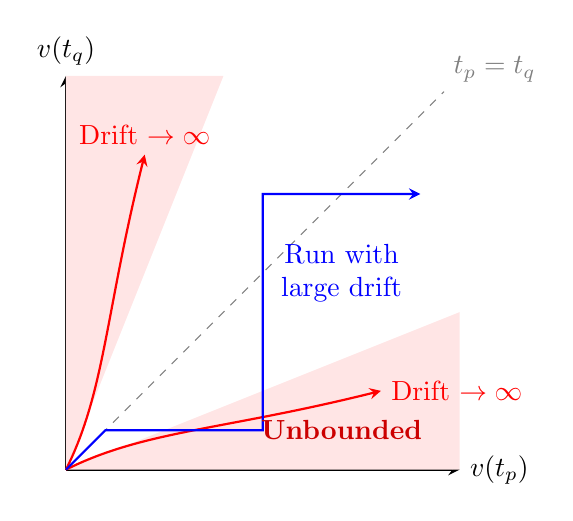
\begin{tikzpicture}[>=stealth]
            % Axes
            \draw[->, thick] (0,0) -- (5,0) node[right] {$v(t_p)$};
            \draw[->, thick] (0,0) -- (0,5) node[above] {$v(t_q)$};
            
            % Diagonal (Reference)
            \draw[dashed, gray] (0,0) -- (4.8,4.8) node[above right] {$t_p = t_q$};
            
            % Unbounded Region
            \fill[red!10] (0,0) -- (5,2) -- (5,0) -- cycle; 
            \fill[red!10] (0,0) -- (2,5) -- (0,5) -- cycle;
            
            \draw[red, thick, ->] (0,0) .. controls (1,0.5) and (2,0.5) .. (4,1) node[right] {Drift $\to \infty$};
            \draw[red, thick, ->] (0,0) .. controls (0.5,1) and (0.5,2) .. (1,4) node[above] {Drift $\to \infty$};
            
            % Sample Run
            \draw[thick, blue, ->] (0,0) -- (0.5, 0.5) -- (2.5, 0.5) -- (2.5, 3.5) -- (4.5, 3.5);
            \node[blue, align=center] at (3.5, 2.5) {Run with\\large drift};
            
            % Annotation
            \node[align=center, text=red!80!black] at (3.5, 0.5) {\textbf{Unbounded}};
        \end{tikzpicture}
        }
        \caption{\textbf{Unbounded Drift.} The difference $|v(t_p) - v(t_q)|$ can grow arbitrarily. Reachable states diverge far from the diagonal $t_p = t_q$, requiring infinite state space to track all possibilities.}
        \label{fig:drift_unbounded}
    \end{subfigure}
    \hfill
    % --- Subfigure 2: Bounded Drift ---
    \begin{subfigure}[b]{0.45\textwidth}
        \centering
        \resizebox{\textwidth}{!}{%
        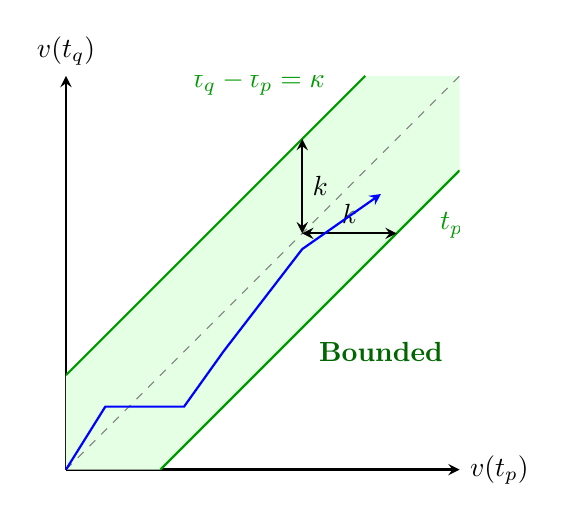
\begin{tikzpicture}[>=stealth]
            % Axes
            \draw[->, thick] (0,0) -- (5,0) node[right] {$v(t_p)$};
            \draw[->, thick] (0,0) -- (0,5) node[above] {$v(t_q)$};
            
            % Definitions
            \def\driftK{1.2}
            
            % The Band
            \begin{scope}
                \clip (0,0) rectangle (5,5);
                
                % Fill the valid band
                \fill[green!10] (0,0) -- (5,5) -- (5-\driftK, 5) -- (0, \driftK) -- cycle;
                \fill[green!10] (0,0) -- (5,5) -- (5, 5-\driftK) -- (\driftK, 0) -- cycle;
                
                % Draw the boundary lines
                \draw[thick, green!60!black] (0, \driftK) -- (5-\driftK, 5) node[pos=0.9, above left] {$t_q - t_p = k$};
                \draw[thick, green!60!black] (\driftK, 0) -- (5, 5-\driftK) node[pos=0.9, below right] {$t_p - t_q = k$};
            \end{scope}
            
            % Diagonal
            \draw[dashed, gray] (0,0) -- (5,5);
            
            % Arrows indicating bound
            \draw[<->, thick] (3,3) -- (3, 3+\driftK) node[midway, right] {$k$};
            \draw[<->, thick] (3,3) -- (3+\driftK, 3) node[midway, above] {$k$};

            % Sample Run
            \draw[thick, blue, ->] (0,0) -- (0.5, 0.8) -- (1.5, 0.8) -- (2.0, 1.5) -- (3.0, 2.8) -- (4.0, 3.5);
            
            % Annotation
            \node[align=center, text=green!40!black] at (4, 1.5) {\textbf{Bounded}};
        \end{tikzpicture}
        }
        \caption{\textbf{Bounded Drift ($k$-bounded).} All reachable configurations satisfy $|v(t_p) - v(t_q)| \le k$. States are confined to a diagonal band of width $2k$, enabling finite region abstraction.}
        \label{fig:drift_bounded}
    \end{subfigure}
    
    \caption{Geometric interpretation of drift in the space of reference clocks. The axes represent reference-clock values $v(t_p)$ and $v(t_q)$ for two agents. Although both values grow unboundedly over time, $k$-drift boundedness constrains their relative positions.}
    \label{fig:drift_comparison}
\end{figure}

Figure~\ref{fig:drift_comparison} visualizes drift in a two-agent system as a trajectory in the $(v(t_p), v(t_q))$ plane. The diagonal $v(t_p) = v(t_q)$ represents perfect synchronization.

\paragraph{Unbounded drift (left).} Without restrictions, executions may diverge arbitrarily far from the diagonal. The reachable region is potentially the entire quadrant, yielding an unbounded two-dimensional state space. This illustrates why standard region abstractions fail: tracking unbounded clock differences requires infinitely many regions, and these differences can encode counter values.

\paragraph{Bounded drift (right).} Under a drift bound $|v(t_p) - v(t_q)| \le k$, reachable configurations are constrained to an infinite strip of fixed width around the diagonal. Although time itself grows unboundedly, the \emph{relative positions} of reference clocks remain bounded. Crucially, this strip can be collapsed into a finite abstraction by quotienting time elapse, which is precisely what the $k$-region construction exploits (Section~\ref{sec:k-regions}).

\subsection{Motivating Examples}

To make drift boundedness concrete, we present two examples that illustrate the difference between unbounded and bounded drift at the level of simple control structures.

\begin{example}[Unbounded vs.\ bounded drift]
\label{ex:drift}
Figure~\ref{fig:abc} shows two LTNs over agents $p$ and $q$ that differ only in their timing constraints and synchronization patterns.

\paragraph{LTN $\Nn_1$ (left): Unbounded drift.} Nodes $n_1$ and $n_2$ both have self-loops labeled $a$ and $b$ respectively, each with guard $x = 1$ (or $y = 1$) and reset set $\{x\}$ (or $\{y\}$). For any $k \ge 0$, agent $p$ can execute the $a$-loop on $n_1$ exactly $k+1$ times while agent $q$ does not execute its $b$-loop at all. At the resulting configuration, node $n_3$ becomes enabled, but the reference-clock difference satisfies
\[
  |v(t_p)-v(t_q)| \;\ge\; k.
\]
Hence, the drift can grow arbitrarily large along reachable configurations.

Moreover, this drift cannot be reduced afterward. If agent $q$ allows more than one unit of local time to elapse while agent $p$ continues executing $a$-loops, then $q$ will violate the guard of its $b$-loop and can no longer perform it. Consequently, any run realizing the word $a^{k+1}b^{k+1}$ necessarily maintains drift at least $k$ throughout its execution, demonstrating that unbounded drift is intrinsic to the system's behavior.

\paragraph{LTN $\Nn_2$ (right): Bounded drift.} The structure is similar, but $\Nn_2$ enforces bounded drift through the time-synchronizing node $n_3$ (shown with a dotted line, indicating synchronization). Whenever $n_3$ is executed, the reference clocks of $p$ and $q$ are synchronized to the same value, so $\drift(v) = 0$ at that point. After synchronization, agent $p$ must wait at least 2 time units before executing $a$ (guard $x \ge 2$), while agent $q$ must execute $b$ within 1 time unit (guard $y \le 1$). This creates a maximum drift of $2 - 1 = 1$.

Repeating this synchronization pattern ensures that all reachable configurations of $\Nn_2$ satisfy $\drift(v) \le 1$, regardless of how many times the agents cycle through their behaviors.

    \begin{figure}[h]
        \centering
        \begin{minipage}{.45\textwidth}
        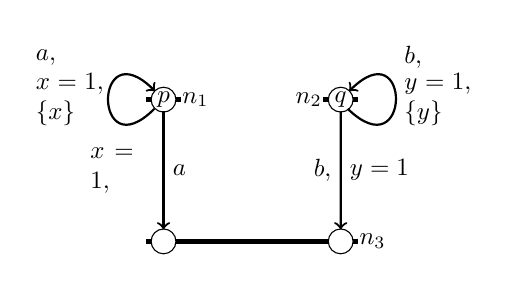
\begin{tikzpicture}[scale=0.9, every node/.style={transform shape}]
        
        \begin{scope}[line width=2pt]
        \draw (-.25,0) -- (0.25,0);
        \draw (2.25,0) -- (2.75,0);
        \draw (-.25,-2) -- (2.75,-2);
        \end{scope}
        
        \filldraw [fill=white]  (0,0)  circle (1.75mm) node (pa) {$p$};
        \filldraw [fill=white]  (2.5,0)  circle (1.75mm) node (qb) {$q$};
        \filldraw [fill=white]  (0,-2)  circle (1.75mm) node (pc) {};
        \filldraw [fill=white]  (2.5,-2)  circle (1.75mm) node (qc) {};
        
        \node at (0.45,0) {$n_1$};
        \node at (2.05,0) {$n_2$};
        \node at (2.95,-2) {$n_3$};
        \node at (-1.3,0.6) [text width=1cm] {$a,$};
        \node at (3.9,0.6) [text width=1cm] {$b,$};
        \node at (-1.3,0) [text width=1cm] {$x=1,$ $\{x\}$};
        \node at (3.9,0) [text width=1cm] {$y=1,$ $\{y\}$};
        
        \begin{scope}[thick,->]
        \draw (pa) + (0,-.165) -- (0,-1.83) node [midway, right] {$a$} node [midway, left, text width=0.9cm] {$x=1,$};
        \draw (qb) + (0,-.165) -- (2.5,-1.83) node [midway, left] {$b,$} node [midway, right, text width = 0.9cm] {$y=1$};
        \draw (-0.13,-0.13) .. controls (-1,-1) and (-1,1) .. (-0.12,0.12);
        \draw (2.6,-0.13) .. controls (3.5,-1) and (3.5,1) .. (2.62,0.12);
        \end{scope}
        
        \end{tikzpicture}
        \end{minipage}
        \begin{minipage}{.45\textwidth}
        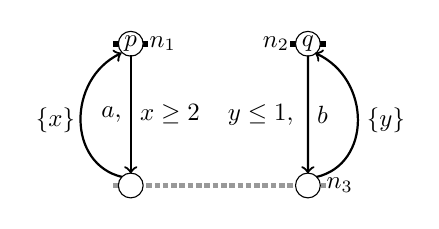
\begin{tikzpicture}[scale=0.9, every node/.style={transform shape}]
        
        \begin{scope}[line width=2pt]
        \draw (-.25,0) -- (0.25,0);
        \draw (2.25,0) -- (2.75,0);
        \draw [opacity=0.4, densely dotted] (-.25,-2) -- (2.75,-2);
        \end{scope}
        
        \filldraw [fill=white]  (0,0)  circle (1.75mm) node (pa) {$p$};
        \filldraw [fill=white]  (2.5,0)  circle (1.75mm) node (qb) {$q$};
        \filldraw [fill=white]  (0,-2)  circle (1.75mm) node (pc) {};
        \filldraw [fill=white]  (2.5,-2)  circle (1.75mm) node (qc) {};
        
        \node at (0.45,0) {$n_1$};
        \node at (2.05,0) {$n_2$};
        \node at (2.95,-2) {$n_3$};
        
        \begin{scope}[thick,->]
        \draw (pa) + (0,-.165) -- (0,-1.83) node [midway, left] {$a,$} node [midway, right, text width=0.85cm] {$x \ge 2$};
        \draw (qb) + (0,-.165) -- (2.5,-1.83) node [midway, right] {$b$} node [midway, left, text width = 1cm] {$y \le 1,$};
        \draw (pc) + (-0.12, 0.12) .. controls (-0.9,-1.7) and (-0.9,-0.5) .. (-0.13, -0.13) node [midway, left, text width=0.5cm] {$\{x\}$};
        \draw (qc) + (0.12, 0.12) .. controls (3.4,-1.7) and (3.4,-0.5) .. (2.6, -0.13) node [midway, right, text width=0.5cm] {$\{y\}$};
        \end{scope}
        
        \end{tikzpicture}
        \end{minipage}
        \caption{LTN $\Nn_1$ with unbounded drift (left) and $1$-drift bounded LTN $\Nn_2$ (right). The dotted line in $\Nn_2$ indicates a synchronizing interaction.}
            \label{fig:abc}
        \end{figure}
\end{example}

\begin{example}[ATM transaction with bounded drift]
\label{ex:atm-bounded-drift}
Consider the ATM transaction LTN from Figure~\ref{fig:ATM} (Chapter~\ref{chap:ltn}) with three agents: customer $c$, ATM $a$, and bank $b$. The negotiation exhibits partial synchronization—some interactions involve all three agents, while others involve only pairs.

\textbf{Claim:} This LTN is 10-drift bounded (assuming appropriate guard constants).

\textbf{Intuition:} 
\begin{itemize}
\item The customer $c$ can delay at most 10 units between interactions (guard $x \leq 10$ at outcome $\mathsf{e\_otp}$).
\item The bank $b$ can delay at most 3 units between interactions (guards $y \leq 3$ at $\mathsf{match}$ and $\mathsf{fail}$).
\item The ATM $a$ coordinates both, so its reference clock stays between $t_c$ and $t_b$.
\item Maximum drift occurs when $c$ is at $t_c = 10$ and $b$ hasn't started ($t_b = 0$), giving $\drift = 10$.
\item Subsequent interactions force resynchronization, preventing unbounded divergence.
\end{itemize}

This example illustrates that drift boundedness is compatible with partial synchronization and does not require the extreme restrictions of synchronization-free or always-synchronizing LTNs.
\end{example}

\subsection{Drift-Bounded Runs and LTNs}

We now formalize drift boundedness for runs and systems.

\begin{definition}[$k$-drift-bounded run]
\label{def:drift-bounded-run}
A run
\[
  \rho = (C_1,v_1)\xra{(\Delta_1,e_1)}(C_2,v_2)\xra{(\Delta_2,e_2)}\cdots
\]
is \emph{$k$-drift bounded} if every configuration $(C_i,v_i)$ occurring in the run satisfies $\drift(v_i) \le k$.
\end{definition}

The central notion studied in this chapter is an \emph{existential}, \emph{retiming-based} boundedness condition, standard in the timed-automata literature.

\begin{definition}[$k$-drift-bounded LTN]
\label{def:retiming-bounded}
An LTN $\Nn$ is \emph{$k$-drift bounded} if for every run
\[
  \rho = (C_1,v_1)\xra{\Delta_1,e_1}(C_2,v_2)\xra{\Delta_2,e_2}\cdots
\]
of $\Nn$, there exists a run
\[
  \rho_k = (C_1,v_1)\xra{\Delta'_1,e_1}(C_2,v'_2)\xra{\Delta'_2,e_2}\cdots
\]
with the same sequence of discrete outcomes $e_1, e_2, \ldots$, obtained by modifying only the local delays, such that $\rho_k$ is $k$-drift bounded.
\end{definition}

Thus, an LTN is $k$-drift bounded if every discrete behavior (untimed sequence of outcomes) admits at least one timed realization in which drift never exceeds~$k$.

\paragraph{Existential vs.\ universal drift boundedness.}
Definition~\ref{def:retiming-bounded} uses an \emph{existential} notion: we require that \emph{some} timed realization of each discrete behavior is drift-bounded, not that \emph{all} realizations are. This is the appropriate notion for reasoning about time-abstract behaviors via retiming and aligns with standard practice in timed automata verification.

In contrast, a \emph{universal} notion would require \emph{every reachable configuration} to satisfy the drift bound. Universal drift boundedness is stronger and less commonly satisfied, but it is also a natural property to verify (see Section~\ref{sec:drift-meta}). Throughout this chapter, "drift-bounded" without qualification means existentially drift-bounded.

\section{The $k$-Drift Bounded Fragment}
\label{sec:k-drift-fragment}

We now establish decidability and complexity for the class of $k$-drift bounded LTNs. The key insight is that bounded drift enables a finite abstraction analogous to region constructions for timed automata.

\subsection{Region Abstraction Under Bounded Drift}
\label{sec:k-regions}

Fix a constant $k\in\Nat$ and let $M$ be the maximum constant appearing in any clock constraint of $\Nn$. We adapt the region equivalence from networks of timed automata~\cite{DBLP:conf/concur/HerbreteauSW22} to LTNs.

\begin{definition}[$k$-Drift region equivalence $\cong_M^k$]
\label{def:k-region-equiv}
Let $M$ be the maximal constant in guards and $k$ the drift bound. Two $k$-drift bounded valuations $v, v'$ are equivalent, written $v \cong_M^k v'$, if:
\begin{enumerate}
    \item \textbf{Integral parts of local clocks:} For all $x \in \bigcup_{p \in P} X_p$, either $\lfloor v(x) \rfloor = \lfloor v'(x) \rfloor$ or both exceed $M$.
    
    \item \textbf{Fractional ordering:} For all clocks $x, y \in \bigcup_{p \in P} (X_p \cup \{t_p\})$, we have $\{v(x)\} \leq \{v(y)\}$ if and only if $\{v'(x)\} \leq \{v'(y)\}$, and equality of fractional parts is preserved: $\{v(x)\} = \{v(y)\}$ iff $\{v'(x)\} = \{v'(y)\}$.
    
    \item \textbf{Reference clock differences:} For all agents $p, q \in P$, we have $\lfloor v(t_p) - v(t_q) \rfloor = \lfloor v'(t_p) - v'(t_q) \rfloor$.
\end{enumerate}
\end{definition}

Although LTNs use explicit local clocks rather than the offset representation common in timed automata, the equivalence $\cong_M^k$ captures the same essential information:
\begin{itemize}
\item Condition (1) abstracts local clock values by their integer parts up to $M$, beyond which guards cease to distinguish values.
\item Condition (2) preserves the ordering of fractional parts, which determines the order in which clocks become integral and thus which guards become enabled.
\item Condition (3) tracks integer differences between reference clocks, which are bounded by $k$ under drift boundedness and determine synchronization constraints.
\end{itemize}

The key property of $\cong_M^k$ is that it is a \emph{time-abstract bisimulation} on the space of $k$-drift-bounded configurations: if $(C,v) \cong_M^k (C,v')$, then
\begin{enumerate}
\item For every local delay $\Delta$ from $(C,v)$, there exists a delay $\Delta'$ from $(C,v')$ such that $(C,v+\Delta) \cong_M^k (C,v'+\Delta')$.
\item $v$ satisfies a guard with constants at most $M$ if and only if $v'$ does.
\item For every synchronizing outcome, the equality constraints $v(t_p) = v(t_q)$ for participants $p, q$ are preserved under equivalent valuations.
\end{enumerate}

Consequently, for every $k$-drift-bounded run starting from $(C,v)$, there exists a $k$-drift-bounded run with the same discrete behavior starting from any $(C,v')$ with $(C,v) \cong_M^k (C,v')$.

\begin{lemma}[Finiteness of $\cong_M^k$]
\label{lem:finite-regions}
The equivalence $\cong_M^k$ has finitely many equivalence classes. Specifically, the number of regions is bounded by
\[
O\bigl( |N| \cdot 2^{|X|} \cdot |X|! \cdot (2M+1)^{|X|} \cdot (2k+1)^{|P|^2} \bigr),
\]
where $|N|$ is the number of nodes, $|X| = \sum_{p \in P} |X_p|$ is the total number of local clocks, and $|P|$ is the number of agents.
\end{lemma}

\begin{proof}
Each region is determined by:
\begin{itemize}
\item A marking $C$ (at most $|N|$ possibilities).
\item Integer parts of local clocks up to $M$ (at most $(M+2)^{|X|}$ possibilities, accounting for values $> M$).
\item An ordering of fractional parts among $|X| + |P|$ clocks (at most $(|X| + |P|)!$ orderings, and $2^{|X|+|P|}$ to record which are zero).
\item Integer differences $\lfloor t_p - t_q \rfloor$ for all pairs, bounded by $k$ (at most $(2k+1)^{|P|^2}$ combinations).
\end{itemize}
The product of these bounds yields an exponential dependence on $|X|$ and $|P|$, but polynomial in $M$ and $k$ when these are treated as parameters.
\end{proof}

\subsection{The $k$-Region Automaton}
\label{sec:k-automaton}

Using equivalence classes of $\cong_M^k$ as states, we construct a finite \emph{$k$-region automaton} $\mathcal{R}_k(\Nn)$ whose transitions abstract both time elapse and discrete outcomes.

\begin{definition}[$k$-Region automaton]
The $k$-region automaton $\mathcal{R}_k(\Nn)$ is a finite automaton with:
\begin{itemize}
\item \textbf{States:} Equivalence classes $[C,v]_{\cong_M^k}$ of $k$-drift bounded configurations.
\item \textbf{Initial state:} $[C_0, v_0]_{\cong_M^k}$ where $(C_0, v_0)$ is the initial configuration.
\item \textbf{Transitions:} $[C,v]_{\cong_M^k} \xrightarrow{e} [C',v']_{\cong_M^k}$ if there exist representatives $(C,v)$ and delays $\Delta, \Delta'$ such that $(C, v + \Delta) \xrightarrow{e} (C', v' + \Delta')$ and both configurations are $k$-drift bounded.
\end{itemize}
\end{definition}

The time-abstract bisimulation property ensures that reachability in $\mathcal{R}_k(\Nn)$ faithfully represents reachability of discrete behaviors in the original LTN.

\begin{theorem}[Soundness and completeness of $\mathcal{R}_k(\Nn)$]
\label{thm:region-automaton-correct}
A marking $C$ is reachable in $\Nn$ via a $k$-drift bounded run if and only if some region $[C,v]_{\cong_M^k}$ is reachable in $\mathcal{R}_k(\Nn)$.
\end{theorem}

\begin{proof}[Proof sketch]
\emph{Soundness:} If $[C,v]_{\cong_M^k}$ is reachable in $\mathcal{R}_k(\Nn)$, then by definition of transitions, there exists a corresponding $k$-drift bounded run in $\Nn$ reaching $(C,v)$.

\emph{Completeness:} If $C$ is reachable via a $k$-drift bounded run $\rho$ in $\Nn$, then by the bisimulation property, there exists an equivalent run through region representatives that witnesses reachability of $[C,v]_{\cong_M^k}$ in $\mathcal{R}_k(\Nn)$.
\end{proof}

\subsection{Decidability and Complexity}
\label{sec:drift-complexity}

We now establish the main complexity result for $k$-drift bounded LTNs.

\begin{theorem}[Main result for drift-bounded LTNs]
\label{thm:drift-pspace}
For each fixed $k \in \mathbb{N}$, location reachability is PSPACE-complete for $k$-drift bounded LTNs.
\end{theorem}

\begin{proof}
\textbf{PSPACE Upper Bound:} 
By Lemma~\ref{lem:finite-regions}, the $k$-region automaton has exponentially many states (in $|X|$ and $|P|$, polynomial in $M$ and $k$). Reachability in this finite automaton can be solved by a nondeterministic algorithm that guesses a path, storing only the current region at each step. This requires polynomial space: $O(\log(|N| \cdot |X|! \cdot M^{|X|} \cdot k^{|P|^2}))$, which is polynomial in the size of the LTN encoding. By Savitch's theorem, NPSPACE = PSPACE, yielding the upper bound.

\textbf{PSPACE Lower Bound:} 
A standard timed automaton $\mathcal{A}$ can be viewed as a single-agent LTN $\Nn_{\mathcal{A}}$. With only one agent, drift is trivially 0 (bounded). Location reachability for timed automata is PSPACE-complete~\cite{AlurDill94}, so reachability in $k$-drift bounded LTNs is PSPACE-hard.
\end{proof}

This result positions drift-bounded LTNs at the same complexity level as timed automata, despite their greater structural flexibility in modeling multi-agent interactions.

\section{Deciding Drift Boundedness}
\label{sec:drift-meta}

A natural meta-question is whether drift boundedness itself can be effectively verified. We consider four variants:

\begin{enumerate}
\item \textbf{Universal $k$-boundedness (fixed $k$):} Given $\Nn$ and $k$, is every reachable configuration $k$-drift bounded?
\item \textbf{Universal boundedness (existence of $k$):} Given $\Nn$, does there exist $k$ such that all reachable configurations are $k$-drift bounded?
\item \textbf{Existential $k$-boundedness (fixed $k$):} Given $\Nn$ and $k$, does every discrete behavior admit a $k$-drift bounded realization? (This is Definition~\ref{def:retiming-bounded}.)
\item \textbf{Existential boundedness (existence of $k$):} Given $\Nn$, does there exist $k$ such that $\Nn$ is existentially $k$-drift bounded?
\end{enumerate}

We address the first two questions here; the existential variants remain open but are less central to practical verification.

\subsection{Universal $k$-Drift Boundedness (Fixed $k$)}

\begin{proposition}[Deciding universal $k$-boundedness]
\label{prop:universal-k-decidable}
Given an LTN $\Nn$ and a constant $k$, deciding whether $\Nn$ is universally $k$-drift bounded is PSPACE-complete.
\end{proposition}

\begin{proof}
\textbf{PSPACE Membership:} 
We reduce this problem to safety reachability over a finite state space. Define an augmented region equivalence $\cong_{M,k}^{\mathrm{univ}}$ that extends $\cong_M^k$ by tracking a special "Unbounded" state reached whenever $|v(t_p) - v(t_q)| > k$ for any pair $p, q$.

Construct a region automaton $\mathcal{R}^{\mathrm{univ}}(\Nn, k)$ over these regions. The LTN violates universal $k$-drift boundedness if and only if the "Unbounded" state is reachable in $\mathcal{R}^{\mathrm{univ}}(\Nn, k)$. Reachability in this finite graph can be checked in NPSPACE, hence PSPACE by Savitch's theorem.

\textbf{PSPACE-hardness:} 
A timed automaton is a single-agent LTN with drift 0. Location reachability for timed automata is PSPACE-complete. We reduce it by adding a self-loop at the target location that enforces large drift (e.g., by having a second dummy agent with an unbounded clock). Reachability of the target in the timed automaton corresponds to reachability of an unbounded-drift state in the constructed LTN.
\end{proof}

\subsection{Universal Drift Boundedness (Existence of $k$)}

\begin{proposition}[Undecidability of universal boundedness]
\label{prop:universal-undecidable}
Given an LTN $\Nn$, it is undecidable whether there exists $k \in \Nat$ such that $\Nn$ is universally $k$-drift bounded.
\end{proposition}

\begin{proof}
In Chapter~\ref{chap:ltn}, it was shown that LTNs can simulate 2-counter machines, where the difference $v(t_p) - v(t_q)$ between reference clocks encodes counter values. Universal drift boundedness is therefore equivalent to asking whether the counters in the simulated machine remain bounded for all possible executions.

The \emph{boundedness problem} for 2-counter machines—determining whether there exists $k$ such that no counter ever exceeds $k$ in any execution—is known to be undecidable~\cite{Minsky67}. Since this problem reduces to checking universal drift boundedness for the corresponding LTN, the latter is also undecidable.
\end{proof}

\section{Acyclic Local-Timed Negotiations}
\label{sec:acyclic}

The results of the previous section establish decidability for $k$-drift bounded LTNs when $k$ is given. However, drift boundedness is a \emph{semantic} property—verifying it requires reasoning about all possible behaviors. A natural question is: when can drift boundedness be guaranteed \emph{structurally}, based solely on the syntax of the LTN?

We now study \emph{acyclic LTNs}, where the absence of cycles in the marking graph implicitly enforces bounded drift, even though acyclicity imposes no explicit constraints on timing or clock values.

\begin{definition}[Acyclic LTN]
\label{def:acyclic-ltn}
A local-timed negotiation $\mathcal{N}$ is \emph{acyclic} if its marking graph contains no cycle.
\end{definition}

In an acyclic LTN, every discrete run visits each marking at most once. This immediately bounds the length of any run by the number of reachable markings, which is finite and computable from the structure of $\Nn$.

\subsection{Acyclicity Implies Drift Boundedness}

\begin{theorem}[Acyclic LTNs are drift bounded]
\label{thm:acyclic-drift-bounded}
Every acyclic local-timed negotiation is existentially drift bounded. Moreover, for every acyclic LTN $\Nn$ there exists a constant $k \in \Nat$, computable from $\Nn$, such that $\Nn$ is $k$-drift bounded.
\end{theorem}

\begin{proof}
Fix an acyclic LTN $\Nn$ over agents $P$ and let $m$ be the maximum length of any discrete run in $\Nn$ (i.e., the maximum number of outcomes in a run). Such an $m$ exists because the marking graph is acyclic, hence every run visits each marking at most once. Clearly, $m \le |N|$ where $|N|$ is the number of nodes.

Let $M$ be the maximum constant occurring in any guard of $\Nn$. We claim that $\Nn$ is $k$-drift bounded for $k := m \cdot (M+1)$.

Consider an arbitrary run
\[
\rho = (C_0,v_0) \xra{\Delta_0,e_0} (C_1,v_1) \xra{\Delta_1,e_1} \cdots \xra{\Delta_{m-1},e_{m-1}} (C_m,v_m).
\]
We construct a retiming $\rho_k$ of $\rho$ that is $k$-drift bounded, proceeding step-by-step.

At step $i$, let $e_i = (n_i, r_i)$ and let $P_i := \dom(n_i)$ be the set of participating agents. Choose the local delays $\Delta'_i = [\delta_{p,i}]_{p \in P}$ as follows:
\begin{itemize}
\item For each participating agent $p \in P_i$, set $\delta_{p,i}$ to be the \emph{least nonnegative} value that enables $e_i$ with respect to $p$ local clocks (after applying previous resets).
\item For each non-participating agent $q \notin P_i$, set $\delta_{q,i} := 0$.
\end{itemize}

These choices preserve the discrete skeleton because enabling of $e_i$ depends only on the clocks of agents in $P_i$. Moreover, by the standard region argument for timed automata, when guards have constants bounded by $M$, the least enabling delay for any agent is strictly less than $M+1$: once a clock exceeds $M$, guards no longer distinguish its precise value, so there always exists an enabling representative with delay $ < M+1$.

Consequently, between two consecutive discrete outcomes, each participating agent advances by at most $M+1$ units of reference time, and non-participants do not advance at all. Since the run has at most $m$ outcomes, for every agent $p$ we have
\[
v_m(t_p) - v_0(t_p) \le m \cdot (M+1) = k.
\]

Because all reference clocks start at the same value in the initial configuration ($v_0(t_p) = 0$ for all $p$), for every pair of agents $p, q \in P$ and every configuration along the retimed run,
\[
|v_i(t_p) - v_i(t_q)| \le m \cdot (M+1) = k.
\]

Thus the retimed run $\rho_k$ is $k$-drift bounded. Since $\rho$ was arbitrary, $\Nn$ is existentially $k$-drift bounded.
\end{proof}

This result is significant because it provides a \emph{syntactic sufficient condition} for a \emph{semantic property}. Acyclicity can be checked efficiently by graph algorithms, yet it guarantees drift boundedness with an explicit, computable bound.

\subsection{NP-Completeness of Reachability}

Having established that acyclic LTNs are drift bounded, we now characterize the complexity of reachability for this fragment.

\begin{theorem}[Reachability for acyclic LTNs]
\label{thm:acyclic-np}
Location reachability for acyclic local-timed negotiations is NP-complete.
\end{theorem}

\begin{proof}
\textbf{NP Membership.} 
Let $\Nn$ be acyclic and let $C_f$ be a target marking. Because the marking graph is acyclic, every discrete run visits each marking at most once, so any run reaching $C_f$ has a discrete skeleton $w = e_0 \cdots e_{m-1}$ of length $m$ bounded by the number of markings.

A nondeterministic algorithm guesses such a sequence $w$ and checks whether it forms a valid path from $C_0$ to $C_f$ in the marking graph. It then verifies whether $w$ admits a timed realization by encoding the problem as a system of difference constraints.

For each agent $p$ and step $i$, introduce variables $t_p^i$ (reference time at step $i$) and $\tilde{x}^i$ (time of last reset for each local clock $x \in X_p$). Guards $x \bowtie c$ at step $i$ become constraints on $t_p^i - \tilde{x}^i$, resets are encoded by equalities $\tilde{x}^{i+1} = t_p^i$ (or $\tilde{x}^{i+1} = \tilde{x}^i$ if not reset), local time elapse by $t_p^{i+1} \ge t_p^i$, and synchronizing outcomes by $t_p^i = t_q^i$ for all participants.

This yields a system $\Phi(w)$ of difference constraints of size polynomial in $m$, $|P|$, and $|X|$. Feasibility of difference constraints can be checked in polynomial time using the Bellman-Ford algorithm. 
Since $m$ is polynomial in the size of $\Nn$ (due to acyclicity), verification is in P. Thus, the overall problem is in NP.

\textbf{NP hardness.} We reduce SUBSET-SUM to reachability in acyclic LTNs. 
Given nonnegative integers $S = \{n_1, \ldots, n_k\}$ and a target $a \in \Nat$, determine whether there exists a subset $I \subseteq \{1, \ldots, k\}$ such that $\sum_{i \in I} n_i = a$.

\textbf{Construction:}
From an instance $(S, a)$, construct a single-agent acyclic LTN $\mathcal{N}_{S,a}$ as follows:
\begin{itemize}
\item Agent set: $\{p\}$.
\item Clock set: $X_p = \{x, y\}$, where $x$ is reset at each stage and $y$ accumulates total elapsed time.
\item Nodes: $\{n_0, n_1, \ldots, n_k, n_f\}$.
\item Initial marking enables $n_0$; target is $n_f$.
\end{itemize}

\textbf{Transitions:}
\begin{itemize}
\item Node $n_0$ has outcome $\mathsf{start}$ with guard $\top$, reset set $\{x\}$, and successor $n_1$.
\item For each $i = 1, \ldots, k$, node $n_i$ has two outcomes:
  \begin{itemize}
  \item \emph{Include} $\mathsf{in}$: guard $(x = n_i)$, reset $\{x\}$, successor $n_{i+1}$ (or $n_f$ if $i = k$).
  \item \emph{Exclude} $\mathsf{out}$: guard $(x = 0)$, reset $\{x\}$, successor $n_{i+1}$ (or $n_f$ if $i = k$).
  \end{itemize}
\item Node $n_f$ has outcome $\mathsf{done}$ with guard $(y = a)$ and no resets.
\end{itemize}

The marking graph forms a linear chain $n_0 \to n_1 \to \cdots \to n_k \to n_f$, hence is acyclic.

\textbf{Correctness:}
At node $n_i$, clock $x$ has just been reset. Outcome $\mathsf{out}$ forces zero delay, while outcome $\mathsf{in}$ forces exactly $n_i$ units of delay. Thus each stage contributes either 0 or $n_i$ time units. Since $y$ is never reset, upon reaching $n_f$ its value equals $\sum_{i \in I} n_i$ where $I$ is the set of indices for which $\mathsf{in}$ was chosen. The final guard $(y = a)$ is enabled iff this sum equals $a$.

Therefore, $n_f$ is reachable iff the SUBSET-SUM instance has a solution. This reduction is polynomial and preserves acyclicity, proving NP-hardness.
\end{proof}

\begin{figure}[t]
\centering
\begin{tikzpicture}[>=stealth, node distance=2.2cm, on grid, auto]

\tikzstyle{node}=[circle, draw, minimum size=7mm]
\tikzstyle{trans}=[->, thick]

\node[node] (n0) {$n_0$};
\node[node, right=of n0] (n1) {$n_1$};
\node[node, right=of n1] (n2) {$n_2$};
\node at ($(n2)+(1.4,0)$) {$\cdots$};
\node[node, right=3.8cm of n2] (nk) {$n_k$};
\node[node, right=of nk] (nf) {$n_f$};

\draw[trans] (n0) -- node[above] {\scriptsize $\mathsf{start},\ R=\{x\}$} (n1);

\draw[trans, bend left=20] (n1) to
node[above] {\scriptsize $\mathsf{in},\ x=n_1,\ R=\{x\}$} (n2);
\draw[trans, bend right=20] (n1) to
node[below] {\scriptsize $\mathsf{out},\ x=0,\ R=\{x\}$} (n2);

\draw[trans, bend left=20] (nk) to
node[above] {\scriptsize $\mathsf{in},\ x=n_k,\ R=\{x\}$} (nf);
\draw[trans, bend right=20] (nk) to
node[below] {\scriptsize $\mathsf{out},\ x=0,\ R=\{x\}$} (nf);

\draw[trans] (nf) -- node[above] {\scriptsize $\mathsf{done},\ y=a$} ++(1.6,0);

\end{tikzpicture}
\caption{Acyclic LTN encoding SUBSET-SUM. Clock $x$ is reset at every step and enforces a choice of delay 0 or $n_i$; clock $y$ accumulates total elapsed time and is checked at the final node.}
\label{fig:subset-sum-ltn}
\end{figure}

The drop from PSPACE (for general $k$-drift bounded LTNs) to NP (for acyclic LTNs) reflects the computational difference between verifying a semantic property versus exploiting a structural guarantee. In acyclic LTNs, the bound on run length provides additional structure that simplifies reachability analysis.

\section{Summary and Perspective}
\label{sec:drift-summary}

This chapter investigated \emph{drift}—the maximum divergence between agents' reference clocks—as both a source of undecidability and a unifying lens for understanding decidable fragments of local-timed negotiations.

\subsection*{Main Contributions}

\paragraph{Semantic restriction: drift boundedness.} We formalized an existential notion of $k$-drift boundedness (Definition~\ref{def:retiming-bounded}), requiring that every discrete behavior admit at least one timed realization with bounded clock divergence. This retiming-based notion, standard in timed automata theory, enables finite abstraction techniques.

\paragraph{Decidability via region abstraction.} For $k$-drift bounded LTNs, we adapted region-equivalence constructions from timed automata to obtain a finite $k$-region automaton (Section~\ref{sec:k-automaton}). This yielded PSPACE-completeness for location reachability (Theorem~\ref{thm:drift-pspace}), matching the complexity of timed automata despite the greater expressiveness of multi-agent interactions.

\paragraph{Structural implication: acyclicity.} We showed that acyclicity of the marking graph—a purely structural, efficiently checkable property—implicitly enforces bounded drift (Theorem~\ref{thm:acyclic-drift-bounded}). For acyclic LTNs, reachability drops to NP-complete (Theorem~\ref{thm:acyclic-np}), reflecting the added structure that simplifies verification.

\paragraph{Meta-complexity.} We established that verifying universal $k$-drift boundedness is PSPACE-complete (Proposition~\ref{prop:universal-k-decidable}), while determining the existence of a universal drift bound is undecidable (Proposition~\ref{prop:universal-undecidable}).

\subsection*{Conceptual Insights}

Three key insights emerge from this chapter:

\begin{enumerate}
\item \textbf{Drift as a unifying principle:} Unbounded drift enables counter encoding and undecidability, while bounded drift—whether enforced semantically or structurally—restores finite abstractions. Both synchronization extremes from Chapter~\ref{chap:fragments} can be understood as special cases where drift is controlled: synchronization-free LTNs trivialize drift by preventing clock comparisons, while always-synchronizing LTNs bound drift through constant resynchronization.

\item \textbf{Existential vs.\ universal:} The existential notion of drift boundedness (retiming-based) is weaker but more useful for verification than universal boundedness. It aligns with time-abstract verification and enables reasoning about discrete behaviors independently of specific timing choices.

\item \textbf{Syntax implies semantics:} Acyclicity provides a syntactic sufficient condition for the semantic property of drift boundedness. This connection is non-obvious—acyclicity constrains control flow but says nothing explicitly about timing—yet it guarantees bounded drift with a computable bound. This pattern suggests that other structural restrictions might similarly imply semantic boundedness properties.
\end{enumerate}

\subsection*{Broader Perspective}

From a broader perspective, this chapter highlights a fundamental trade-off in real-time concurrent systems: expressiveness arises from the combination of local autonomy (independent clocks), selective coordination (partial synchronization), and unbounded temporal evolution, while decidability is recovered by constraining how divergence accumulates across interactions.

The dichotomy between NP (acyclic) and PSPACE (general $k$-drift bounded) also reveals a computational spectrum: systems where boundedness is structurally guaranteed admit simpler verification than those where boundedness must be checked semantically. This suggests that identifying richer classes of structurally drift-bounded LTNs could yield practical decidable fragments.

\section{Coming Next: Connected Communication}
\label{sec:drift-next}

Acyclicity is a strong restriction: many natural systems exhibit cycles in their control structure while still maintaining disciplined patterns of communication and synchronization. The next chapter studies such systems through the notion of \emph{connectedly communicating local-timed negotiations}.

Connectedly communicating LTNs allow cycles in the marking graph but impose a structural constraint on how agents interact across these cycles. Intuitively, agents that diverge in time cannot later compare their clocks without passing through a communication path that enforces synchronization. This condition rules out the counter-encoding patterns responsible for undecidability while retaining significantly more expressive power than acyclic LTNs.

In Chapter~\ref{chap:connected-communication}, we show that connected communication suffices to bound drift and yields decidable reachability, thereby bridging the gap between purely semantic drift bounds (this chapter) and purely structural acyclicity. This completes our characterization of the decidability landscape for LTNs, delineating the boundary between tractable and intractable fragments based on the interplay of timing, synchronization, and interaction structure.